
\chapter {Theoretical Background}
\label{ch:TheoreticalBackground}

This chapter includes the theoretical background for this work discussing related concepts in Computational Fluid Dynamics and Deep Learning.

%----------------------
\section{Fluid dynamics and Navier-Stokes equations}
\label{sec:FluidDynamicsAndNavier-StokesEquations} 
%----------------------

Fluid dynamics is the branch of physics that studies the motion of fluids, both liquids and gases and their interactions with solid boundaries and other fluids. It encompasses a wide range of phenomena, from the flow of water in rivers and the atmosphere's motion to blood circulation in organisms and the behavior of fluids in engineering systems.

The Navier-Stokes equations (See Equations~\ref{eq:navier-stokes}) are fundamental partial differential equations governing the motion of viscous fluids. They describe how fluid velocity, pressure, density, and viscosity evolve over time in response to external forces. The equations are derived from Newton's second law of motion, conservation of mass, and conservation of momentum principles.

The equations consist of two main components: 1) the continuity equation, which represents the conservation of mass, and 2) the conservation of momentum equation, derived from Newton's second law, which describes how the velocity of the fluid changes in response to external forces and internal forces (pressure and viscosity). This is defined in Equation~\ref{eq:navier-stokes} with $t$ time, $\rho$ density, $u$ velocity, $p$ pressure, $\mu$ viscosity, and $F$ external forces.

\begin{equation}
    \begin{aligned}
        \nabla \cdot u &= 0 \\
        \rho(\frac{\partial u}{\partial t} + (u\cdot\nabla)u) &= -\nabla p + \mu \nabla^2 u + \rho F
    \end{aligned}
    \label{eq:navier-stokes}
\end{equation}

The Navier-Stokes equations are nonlinear, leading to complex and sometimes chaotic behavior, such as turbulence. Despite their simplicity, solving these equations analytically for many practical problems is often impossible, leading to the widespread use of numerical methods.

The Navier-Stokes equations have vast applications in various fields, including engineering, meteorology, oceanography. They support the design of aircraft, ships, and vehicles, studying weather patterns, and understanding fluid flow in pipes and channels. However, many fundamental aspects of these equations, including turbulence, remain unsolved problems in mathematics and physics.

%----------------------
\section{Turbulent flow and Reynolds number}
\label{sec:TurbulentFlowAndReynoldsNumber} 
%----------------------

Turbulent flow is characterized by chaotic and unpredictable fluid motion, with irregular fluctuations in velocity, pressure, and flow patterns. It occurs when inertial forces dominate over viscous forces, leading to mixing and eddy formation. The Reynolds number (Re) is a dimensionless parameter that characterizes the flow regime of a fluid. When Re is high, it is a turbulent flow, indicated by the visual appearance of swirling patterns (or eddies), while low Re values indicate a laminar flow type, recognized by a "smooth" flow of the fluid. Thus, turbulent flow is directly correlated to Reynolds numbers, with higher Re values corresponding to more turbulent behavior and lower Re values indicating laminar flow. Equation~\ref{eq:reynolds-numbers} defines Re, with $\rho$ fluid density, L length scale, U velocity, and $\mu$ viscosity.

\begin{equation}
    Re = \frac{\rho LU}{\mu}
    \label{eq:reynolds-numbers}
\end{equation}

%----------------------
\section{Direct Numerical Simulations, RANS and LES}
\label{sec:DirectNumericalSimulationsRANSAndLES} 
%----------------------

In computational fluid dynamics (CFD), Direct Numerical Simulation (DNS), Reynolds-Averaged Navier-Stokes (RANS), and Large Eddy Simulation (LES) are three common approaches for simulating fluid flows, each with its own set of advantages and limitations.

DNS directly solves the Navier-Stokes equations without any modeling assumptions, providing detailed information on all scales of motion in the flow. However, DNS requires high computational resources and is typically only feasible for relatively low Reynolds number flows due to its high computational cost scaling with the cube of the Reynolds number.

RANS averages the Navier-Stokes equations over time to obtain mean flow quantities and then models the effects of turbulent fluctuations using empirical turbulence models. RANS is computationally less expensive than DNS and is suitable for a wide range of engineering applications. However, RANS relies on turbulence models that introduce modeling errors and uncertainties, particularly for complex flows.

LES resolves large-scale turbulent structures explicitly while modeling the effects of smaller-scale turbulence. It strikes a balance between the accuracy of DNS and the computational cost of RANS, making it suitable for simulating moderately high Reynolds number flows. LES captures the essential features of turbulence while reducing modeling errors compared to RANS.

\begin{figure}[H]
    \centering
    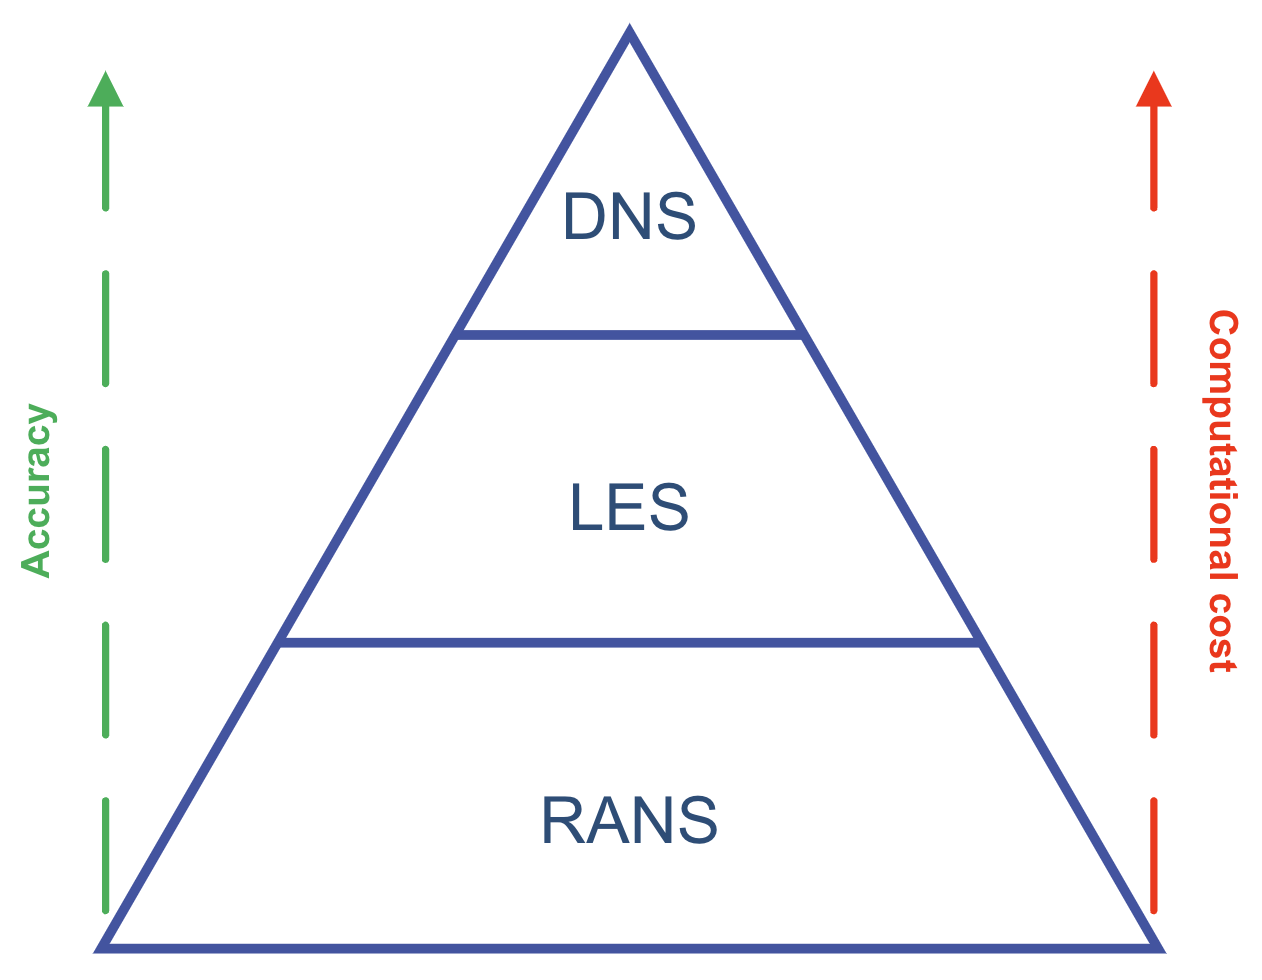
\includegraphics[width=0.4\linewidth]{images/dns_les_rans.png}
    \caption{Comparison between DNS, LES, and RANS modeling}
    \label{fig:dns_les_rans}
\end{figure}

The choice between DNS, RANS, and LES depends on the flow's specific characteristics, the desired detail level, and the available computational resources. Figure~\ref{fig:dns_les_rans} shows a comparison between the different modeling approaches. DNS provides the most accurate results but is computationally expensive, while RANS and LES offer compromises between accuracy and computational cost, making them more practical for many engineering applications.

%----------------------
\section{Time series}
\label{sec:TimeSeries} 
%----------------------

Time Series is a type of data that presents a temporal ordering. It is used in many real-world applications, such as signal processing, finance, weather forecasting, control engineering, communication, human activity recognition, cyber-security, or earthquake prediction. Time series can be described as univariate or multidimensional. Univariate or 1-dimensional time series is an ordered set of real values $X$ of length equal to the number of real values $T$, where $X = [x_1, x_2, ..., x_T]$. While a multidimensional or M-dimensional time series consists of M different univariate time series, where $X = [X^1, X^2, ..., X^M]$ with $X^i \in \mathbb{R}^T$. A Time Series Dataset is defined as $D = \{(X_1, Y_1), (X_2, Y_2), ..., (X_N, Y_N)\}$ as a collection of pairs $(X_i, Y_i)$ where $X_i$ could be a 1-dimensional or M-dimensional time series and an output $Y_i$.

%----------------------
\section{LSTM}
\label{sec:LSTM} 
%----------------------

Recurrent Neural Networks (RNN) are a type of neural network that can keep information about what happened before, they do this with loop connections to their neurons. These neural networks are widely used in speech recognition, language modeling, translation, etc. The main problem with this simple architecture is with “long-term dependencies” when the relevant information happened too long ago. Long Short Term Memory (LSTM) networks are designed to learn long-term dependencies to overcome this issue. The main idea behind the LSTM structure is a memory cell that can accumulate information that can be written and cleared by structures called gates. Fully Connected LSTM (FC-LSTM) is a multivariate version of LSTM, meaning that the input, output, and state are all 1-dimensional vectors.

LSTM neural networks are widely used in Natural Language Processing (NLP), where a long sequence of words in a text needs to be analyzed and used for prediction and classification.

%----------------------
\section{Convolutional Neural Networks}
\label{sec:CNN}
%----------------------

Convolutional Neural Networks (CNN) are a type of neural network primarily designed to process and analyze data in a grid-like organization, especially visual data such as images. Inspired by the organization of the animal visual cortex in the brain, CNNs have been successful in computer vision applications. The key operation in CNNs is the convolution mathematical operation, a specialized kind of linear operation. These networks have a structure called filters, which are applied to the input data to extract features, allowing the neural network to learn hierarchical representations.

CNNs have become the cornerstone of various computer vision tasks, including image classification, object detection, facial recognition, and medical image analysis. Their ability to automatically learn relevant features from raw data makes them particularly effective in tasks where traditional algorithms struggle, such as image understanding and pattern recognition. Additionally, CNNs offer advantages such as parameter sharing, which reduces the number of parameters and enhances model efficiency and translational invariance, enabling robust performance even with variations in object position within an image. Overall, CNNs have revolutionized the field of computer vision and continue to drive advancements in artificial intelligence and image processing applications.

%----------------------
\section{ConvLSTM}
\label{sec:ConvLSTM} 
%----------------------

LSTM neural networks are good for long-time series prediction because they are designed to maintain a context memory of important information that happened long ago as well as recent information. In applications with many dimensions, like spatial data, using an LSTM is inefficient as it contains too much redundancy in the connections between the input. 

ConvLSTM extends the Long Short-Term Memory (LSTM) architecture, incorporating convolutional operations within the LSTM units. It is specifically designed to handle spatiotemporal data, such as video sequences or spatial-temporal patterns in data. ConvLSTM preserves the sequential memory capabilities of LSTM while exploiting the spatial information in data through convolutions. This allows it to capture both temporal dependencies and spatial correlations simultaneously, making it ideal for tasks like video prediction, precipitation nowcasting, and motion tracking. Compared to traditional LSTMs, ConvLSTMs excel in modeling spatial dependencies within sequences, enabling more accurate predictions and better handling of spatially structured data.

%----------------------
\section{Autoencoders}
\label{sec:Autoencoders} 
%----------------------

Autoencoders are an artificial neural network used for unsupervised learning tasks, particularly in dimensionality reduction and data compression. Comprising an encoder and a decoder, they aim to reconstruct input data while learning efficient representations. The encoder compresses the input into a lower-dimensional latent space, while the decoder reconstructs the original data from this representation. Advantages include their ability to learn meaningful representations from unlabeled data, aiding in feature extraction and data denoising. They are widely used in anomaly detection, image denoising, and data generation tasks. Additionally, autoencoders can serve as the foundation for generative models, such as variational autoencoders (VAEs) and generative adversarial networks (GANs), enabling the synthesis of new data samples. Their versatility, simplicity, and capability to learn compact representations make them valuable tools in various domains, including computer vision and natural language processing.

